% -------------------------------------------------------------------------------------------------
% ------------------------------------------ RESULTS --------------------------------------------
% -------------------------------------------------------------------------------------------------
\chapter{Results}
\label{results}

\pagestyle{fancy}

\fancypagestyle{plain}{
\fancyhf{} 
\fancyfoot[RO, LE]{\thepage} 
\renewcommand{\headrulewidth}{0pt}}

\fancyhf{}
\fancyhead[RO, LE]{Results}
\fancyfoot[RO, LE]{\thepage}

\section{Dataset Generation}
For accurate benchmarking of the potentials, the benchmark set used to test the performance of the potentials should be similar to the dataset the statistical potentials were trained on. Since the Buried Surface Area (BSA) of the complex was used as a filtration parameter, the frequency distributions of BSA were compared in the two sets to check for similarity (Figure \ref{SASA_plot}). The BSA values for the 3764 structures in the training set and the 296 structures in the benchmark are similarly distributed. The Mean and Median values for the training set were 1279.5 and 1190.2 respectively, whereas the Mean and Median values for the benchmark set were 1279.5 and 1203.67 respectively.

\par
Among the six ways of classifying protein interactions mentioned in the Introductions section (Sec \ref{interface_prop}), four categories (obligate, non-obligate, transient and permanent) pertain to the dynamics of protein complexes and it is not possible for us to retrieve this information from the crystal structures of proteins (though some of the studies may include information about the kind of interface, overall such studies are sparse). Concerning the oligomeric state of the protein complexes, we find that 90 \% (3389 out of 3764) of the structures in the training set are homodimers. Similarly, 88 \% (264 out of 300) of the structures in the testing set are homodimers.

\section{Benchmarking of the Two-Body Potentials}
The performance of the different statistical potentials was compared using two different methods.
\begin{enumerate}
\item Receiver-Operating Characteristic Curves for different Z-score thresholds
\item Rank - Ordering the scores of the native structures against scores from a randomized background set.
\end{enumerate} 

\vfill

\begin{figure}
	\centering
	\subfloat[The BSA distribution for the training set]{\includegraphics[width=0.75\linewidth,scale=0.3]{./results/train_SASA.eps}}\\
	\subfloat[The BSA distribution for the testing set]{\includegraphics[width=0.75\linewidth,scale=0.3]{./results/test_SASA.eps}}
	\caption[BSA Distributions for training and testing sets]{Histograms depicting the distribution of the Buried Surface Area (BSA) for protein complexes in both the training and the testing set. The number of structures in the training and the testing sets are 3764 and 296 respectively. The binwidth used for plotting the distribution was 25. The red and blue lines on the plot represent the mean and the median of the distributions respectively. The black curve with grey shading is the kernel density estimation for the distribution.}
	\label{SASA_plot}
\end{figure}

\subsection{Benchmarking using ROC curves}
The testing of the 96 different statistical potentials was done on a benchmark set of 296 dimers and their performance was compared using ROC curves. The potentials showed a diverse range of performances as can be seen in Figure \ref{multi-ROC}. 11 of the 96 potentials had an Area Under the Curve of their ROC curves greater than 0.90 (shown in the inset of Fig \ref{multi-ROC}). All eleven of these potentials were variants of the side chain-side chain potentials that were weighted by $cifa$. The main chain-main chain potentials were the worst performers of all with some of the potentials performing worse than a random classifier.
\par The highest power of discrimination between the native and non-native interfaces was achieved by the statistical potential built from side chain-side chain interactions across the interface at the threshold distance of 4 \AA \;(4.ss.norm.cifa.avg in Figure \ref{multi-ROC}). The weighting parameter for this potential was $cifa$, calculated at a single distance of 4 \AA \; and the reference state was weighted by the average weight for residue pairs in the dataset. The area under the curve (AUC) for the ROC curve for this potential was 0.9622. The true positive rates and the false positive rates at the optimal Z-score of -0.7 were 97.8\%  and \% respectively. 

\begin{figure}[ht]
	\centering
	\includegraphics[width=\textwidth, height=\textheight, keepaspectratio]{./results/all_roc_charac.eps}
	\caption[ROC curves for the pairwise potentials]{A comparison of the performances of the 96 different potentials as represented by their Receiver-Operator curves. \textbf{Inset}: Zoomed in version for the best performing potentials. }
	\label{multi-ROC}
\end{figure}

\vfill

\subsection{Benchmarking using Rank Ordering}
After rank ordering the scores of the native and the decoy confirmations, the number of cases where the native confirmation had the best score was also used to compare the performance of the different potentials. On the basis of the interacting atoms, the performance of the potentials was in the order: side chain-side chain > all atoms > main chain-side chain > main chain-main chain (Fig \ref{inter_type}). The performance of the potentials based on the nature of the weights (i.e. whether they were computed at a single distance (norm) or computed as an average from three different distances (avg)) was comparable across the different potentials. Only in the case of the potentials constructed at the distance threshold of 4 \AA \; side chain-side chain potential, is the norm potential better than cmpd potential.

\begin{figure}[ht]
	\centering
	\includegraphics[width=\textwidth, keepaspectratio]{./results/FP_inter_type.eps}
	\caption[Pairwise potential performance based on interacting atom types]{A comparison of the performances of the different potentials as measured by the number of native structures that were ranked 1 against a set of decoy structures. The different facets in the figure describe the performances of the potentials according to the interacting atoms type (all - all atom, mm - main chain-main chain, ms - main chain-side chain and ss - side chain-side chain). The colors differentiate between the potentials based on the nature of the weights, red for cmpd (weight computed as an average at three distances) and cyan for norm (weight computed at a single distance)}
	\label{inter_type}
\end{figure}

The performances of the potentials followed a similar pattern when dissected according to  the distance threshold (Fig \ref{pot_type}). The $cifa$ potential performed better than the $ipa$ potential in all cases. Here again, the side chain-side chain potential at 4 \AA \; with $cifa$ as the weighting parameter computed at a single distance (4.ss.norm.cifa.avg) was the best performer. 137 out of 296 native structures were best ranked when compared against their randomised backgrounds and 240 structures out of 296 have their native structures ranked under 25.

\begin{figure}[H]
	\centering
	\includegraphics[width=\textwidth, keepaspectratio]{./results/FP_weight_type.eps}
	\caption[Pairwise potential performance based on distance threshold]{A comparison of the performances of the different potentials as measured by the number of native structures that were ranked 1 against a set of decoy structures. The graph is dissected based on threshold interaction distance and the different potential type; cyan represents the $ipa$ potential whereas red stands for the $cifa$ potential.}
	\label{pot_type}
\end{figure}

\par 
The potentials with an Area Under the ROC Curve (AUC) greater than 0.90 were checked for complementarity in terms of protein complex prediction (whether different protein complexes were ranked best by different potentials). The results are summarised in Table \ref{complement}. The union of the best ranked sets (set of structures whose native structures were ranked 1 against a randomised background) for the different potentials was greater than the best ranked set for the best performing statistical potential (4.ss.norm.cifa.avg).

\begin{center}
	\begin{tabular}{ | c | c | c | }
	\hline
	cut\_off rank & best performing potential (4.ss.norm.cifa.avg) & Union of AUC $\geq$ 0.9 \\ \hline
	$\leq$ 0 & 137 & 169 \\ \hline
	$\leq$ 5 & 190 & 217 \\ \hline
	$\leq$ 10 & 216 & 235 \\ \hline
	$\leq$ 15 & 224 & 247 \\ \hline
	$\leq$ 20 & 233 & 252 \\ \hline
	$\leq$ 25 & 239 & 261 \\ \hline
	\end{tabular}
	\captionof{table}{Complementarity between the different potentials at different rank cut-offs. The number of structures that were ranked 1 against their respective backgrounds for the two cases are given in the two columns.}
	\label{complement}
\end{center}

There is a preference for same-interaction pairs and complementarity between opposite charges (eg Lysine pairing up favourably with Glutamate and Aspartate) is also observed in the log-odds ratio matrix (Fig \ref{score_matrix}). Cysteine-Cysteine and Histidine-Histidine are among the best scored residue residue contact pairs. The contact preference scores for the hydrophobic amino acids are overall favourable though any specific preferences are not observed.

\begin{figure}[ht]
	\centering
	\includegraphics[scale = 0.3]{./results/score_matrix.eps}
	\caption[Log odds ratio matrix of Residue Pair preferences in pairwise potential]{Log odds ratio of residue pair preferences across protein - protein interfaces for the best two-body potential. The darker the shade, the higher the preference}
	\label{score_matrix}
\end{figure}

\subsection{Testing Potential Values for GLY-GLY pairs}
Since, Glycine lacks a side chain, the potential values for GLY-GLY pairs for the side chain-side chain potentials were tested as described in Methods. For the side-chain potentials at 4 and 8 \AA \;, assuming that the occurrence of Glycines on the interface is random (column no-effect in Table \ref{GLY_table}), gave the best performance. For the potential at 6 \AA, \; however, the assumption that GLY residues are unfavourable worked the best.

\begin{center}
	\begin{tabular}{ | c | c | c | c |}
	\hline
	potentials & all atom potentials & unfavourable score (1.38) & no-effect (0.00) \\ \hline
	4.ss.norm.cifa.avg & 109 & 132 & 136 \\ \hline
	6.ss.norm.cifa.avg & 100 & 131 & 113 \\ \hline
	8.ss.norm.cifa.avg & 91 & 99 & 110 \\ \hline
	\end{tabular}
	\captionof{table}{Testing of side chain-side chain potential values for GLY-GLY pairs: Native confirmation scores were rank ordered against decoy conformation scores and the number of structures with native confirmations as best ranked was noted}
	\label{GLY_table}
\end{center}

\vfill

\subsection{Performance on the testing set}
With a Z-score threshold of -0.7 for the best pairwise potential (4.ss.norm.cifa.avg), 284 out of the 295 native structures testing set had a z-score below the threshold, which corresponds to a true prediction. Among the 11 structures which had a z-score greater than the threshold, 7 structures were incorrectly submitted as dimers in the PDB. The biological assemblies for these structures (PDB codes: 3PNA, 1IFQ, 3MTX, 1PL3, 3QL9, 4CMP, 2XRW) is a monomeric entity, as given in the Protein Data Bank. These false classifications in the PDB may be a result of crystallization artefacts. Since, our potentials could successfully distinguish crystal artefacts from true interactions, these 7 structures were considered as correct predictions. Hence, our potentials could correctly identify 291 out of 295 structures, which translates to a prediction accuracy of 98.6 \%.

\subsection{Comparison with MODTIE}
The performance of the best performer was compared with MODTIE \citep{Davis2006} (Fig \ref{compare_modtie}). Benchmarking for both the potentials was done on the same benchmark set. The Area under the curve for the MODTIE potential was 0.9445. The true positive rate and the false positive rate at the Z-score threshold of -1.7 was 71.5 \% (211/295) and 28.5 \% (84/295) respectively.
\begin{figure}[H]
	\centering
	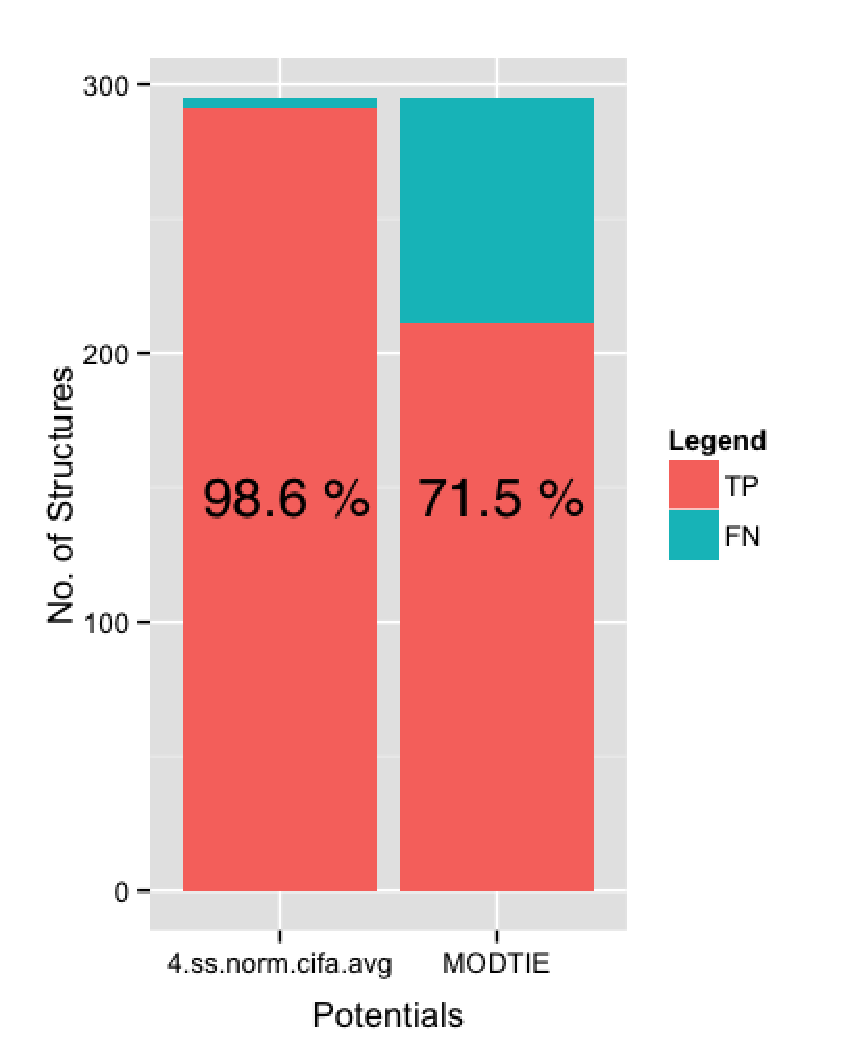
\includegraphics[scale = 0.3]{./results/modtie_TP.eps}
	\caption[Comparison between MODTIE and our potentials]{Performance of the two body potential in comparison to MODTIE. The red part  and the cyan part of the plot depict the no. of True Positives and the no. of False Negatives respectively.}
	\label{compare_modtie}
\end{figure}

\subsection{Multibody Potentials}
The performance of the multi body potentials was accessed in a manner similar to the two-body potentials. For case $(i)$, with the intra-domain distance threshold as 5 \AA \; and the intra-domain distance threshold as 8.5 \AA, \; a total of 280114 distinct cliques were observed, out of 323400 distinct possibilities. The Receiver Operating Curve is shown in Fig \ref{ROC_mb}. The Area Under the Curve for the ROC of the potential without any weights was 0.3089, whereas the Area Under the Curve for the potential with the weights was 0.41006. Both the potentials performed worse than a random classifier. \\[36pt]

\begin{figure}[H]
	\centering
	\includegraphics[width=\textwidth, keepaspectratio]{./results/ROC_mb.eps}
	\caption[ROC curves for multi-body potentials]{Performance of the multibody potentials as assessed by the ROC curves. The cyan curve represents the ROC for the unweighted 5-body potential whereas the red curve depicts the ROC for the weighted 5-body potential.}
	\label{ROC_mb}
\end{figure}

\section{Validation}
The potential 4.ss.norm.cifa.avg was tested for its prediction power on the Ral-GEF system. Six variants of GEF were tested for binding with Ral. Experimental evidence shows that four of these variants (RGL1, RGL2, RGL3 and RALGDS) bind Ral in a particular mode, while the other two variants weakly interact with Ral, binding in a different mode. The Z-scores for all the GEFs were below the threshold and hence all six variants are predicted to bind.
\par
Based on the statistical potential scores, we predicted the following hotspot residues, SER:173:A, GLU:34:A, LYS:370:B, ARG:322:B, ARG:42:A and ARG:74:A, in RGL1-Ral complex that upon mutation would weaken the interaction between RGL1 and Ral. These hotspot residues lie in complementary clusters (Fig \ref{hotspot}) and hence mutating them to other residues would lead to unfavourable interactions, thereby weakening the interaction between RGL1 and Ral. \\ [48pt]

\begin{center}
\begin{tabular}{ | c | c | }
	\hline
	\textbf{GEFs} & \textbf{Z-scores} \\ \hline\hline
	\textbf{RALGDS} & -3.59 \\ \hline
	\textbf{RALGPS1} & -3.39 \\ \hline
	\textbf{RALGPS2} & -3.72 \\ \hline
	\textbf{RGL1} & -3.21\\ \hline
	\textbf{RGL2} & -3.11 \\ \hline
	\textbf{RGL3} & -2.72 \\ \hline
	\end{tabular}
	\captionof{table}{The predictions regarding the binding of Ral to GEF variants using the pairwise statistical potentials.}
\end{center}

\begin{figure}[ht]
	\centering
	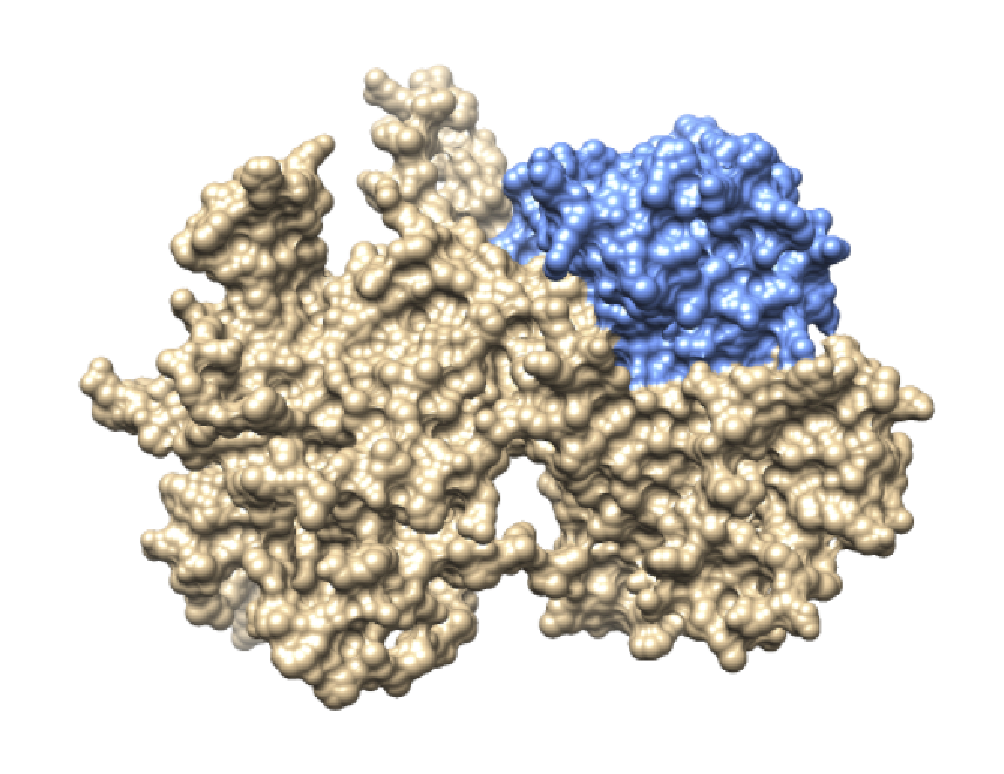
\includegraphics[scale = 0.7]{./results/ralgds1.eps}
	\caption[The RalGDS-Ral complex]{The RalGDS-Ral complex. The Ral subunit is shown in blue in surface representation whereas the RalGDS is depicted in brown, also in surface representation. Image rendered using Chimera \citep{Pettersen2004}}
\end{figure}

\begin{figure}[ht]
\centering
	\subfloat[][Interaction cluster of SER173 of Ral]
	{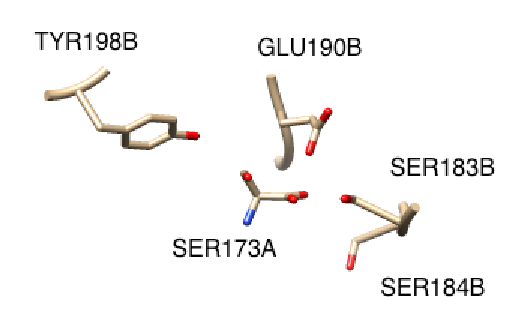
\includegraphics[width = 0.38\linewidth, height = 10em]{./results/ser_rgl1.eps}}
	\hspace{2cm}
	\subfloat[][Interaction cluster of LYS370 of RGL1]
	{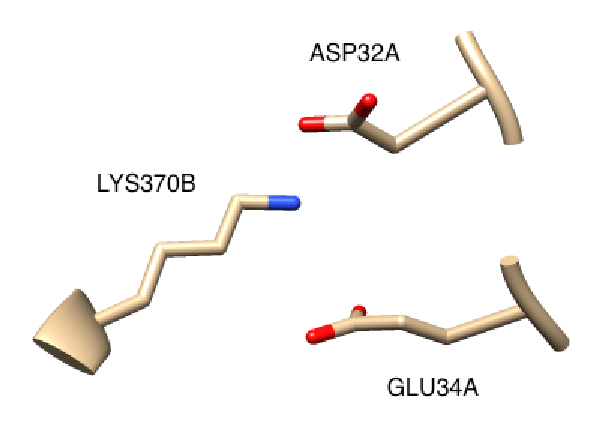
\includegraphics[width = 0.38\linewidth, height = 10em]{./results/lys_rgl1.eps}}
	\caption[Hotspot residues in RGL1-Ral]{Hotspot residues in the RGL1-Ral Complex. Subunit A is Ral and Subunit B is RGL1. Image rendered using Chimera \citep{Pettersen2004}}
	\label{hotspot}
\end{figure}

%%
% -------------------------------------------------------------------------------------------------
% ------------------------------------------ RESULTS --------------------------------------------
% -------------------------------------------------------------------------------------------------